\chapter{绪论}
%
\section{研究背景和意义}
\subsection{研究背景及意义}
打造一个既能看得见,又能听会说Ai的模型一直是人工智能领域的追求。这样的模型可以与人类进行更自然和高效的交互,提供近乎真实的人机交互体验。在过去几十年的发展中,AI技术在视觉、语音、自然语言处理等方面取得了巨大进展,其中视觉问答(VQA)技术尤为重要。
通过VQA技术\cite{yu2015visual},计算机可以像人类一样理解图像内容并回答相关问题\cite{wu2017visual},这为人机交互提供了全新的思路和方式。

随着人工智能技术和视觉问答技术的不断迭代和发展,医学视觉问答(Med-VQA)技术已经作为视觉问答在医学领域的应用而出现,在医学领域中,对医学图像进行分析并回答与之相关的问题。近年来,由于VQA系统在医疗诊断、治疗和教育方面的潜力,该领域吸引了大量关注。
Med-VQA的一个关键挑战是医学图像和问题的复杂性,这通常需要对医学概念和背景有更深入的理解。Med-VQA还需要用到不同的模式信息,如视觉、文本和医学知识。
为了应对这些挑战,该领域的研究人员应用了各种机器学习技术,包括如卷积神经网络(CNN)、递归神经网络(RNN、LSTM)和注意力机制等方法。为此,学者们还探索了不同的模式及其融合手段,包括图像-文本之间的跨模态融合以及从外部引入知识图谱,增加知识图推理等。
Med-VQA有许多潜在的应用,如图\ref{sys_medaicloud}所示,包括为社会构筑完整的智慧医疗体系,协助放射科医生进行诊断、改善医学教育和协助医学研究等。随着Ai、深度学习技术的融入以及在该领域的不断发展,预计未来将会对整个医疗卫生行业产生重要影响。
\begin{figure}[htbp]
	% 图片居中(列居中对齐)
	\centering	
	% 包含当前路径下的Fig文件夹的图片文件
	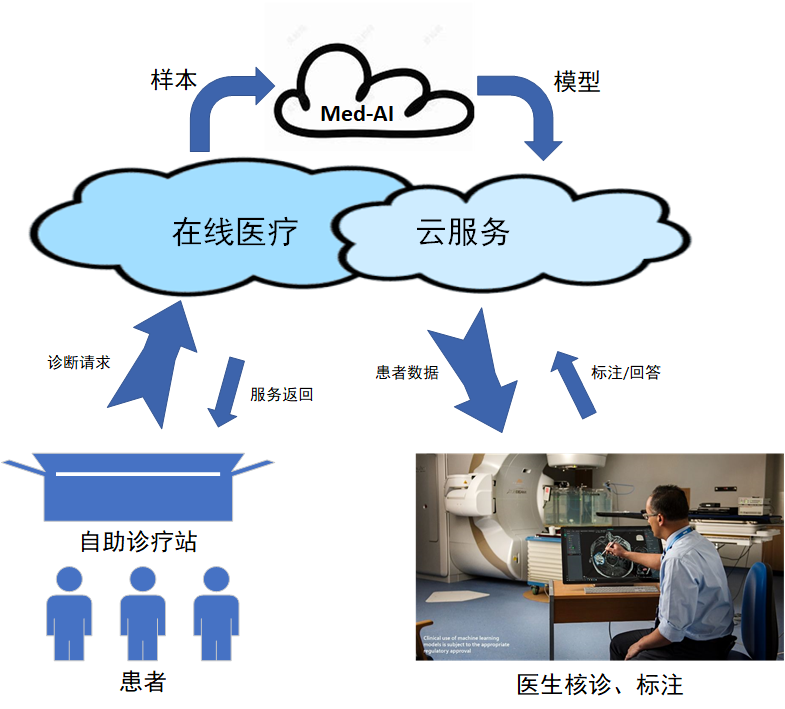
\includegraphics[width=0.8\textwidth]{Fig/myfig/chapter1/sys_medaicloud.png}  %scale = 0.3
	% 添加标签one_DFUAV以及图标题“XXX”,引用某图时使用\ref{xxx},其中xxx就是标签,图编号是自动生成的。
	\caption{\label{sys_medaicloud}AI智慧医疗体系} 
\end{figure}

虽然最早的视觉问答研究是针对通用场景提出的,但人们逐渐发现,相比与让模型去学习通用的“常识”,学习一些专业性更高,更复杂的能力显然更有实际的价值和意义。
所以由VQA技术作为基础,衍生了一系列的子领域以及相关应用。根据QJ WU等人\cite{wu2017visual}的调查,VQA领域的应用大致可以分成5大类,包括基于自然场景的、基于医学图像的、基于人机交互的、
基于图像理解的和其他领域的视觉问答应用:如游戏、社交媒体和虚拟现实等。其中,基于医学图像的视觉问答问答是最具有落地潜力的现实意义方向之一,研究人员正在努力开发一套准确,可靠,丰富
的医学视觉问答系统。例如,在这个应用中,用户可以通过在线的方式实现全自动就医,自助挂号,自助诊查,自助问询,Ai辅助医生完成线上合诊等。医学视觉问答模型的加入可以极大减轻医生的工作负担,降低误诊率,
缩减患者挂号排队问询的流程,提高医院的运行效率。

目前医学视觉问答是一个蓬勃发展的领域,包含计算机科学,生物学,医学,认知科学,心理学等领域等等多学科的研究。从问诊到给患者提供更多的就医服务以及
创造新应用,这个技术的出现会给现有医疗体系变革带来重大且深远的影响。因此可以说,医学视觉问答具有非常重要的研究意义和应用价值。

%
\section{医学视觉问答研究现状}
视觉问答的概念最早在2015年,由斯坦福大学的Licheng Yu等人提出\cite{yu2015visual}并构建了一个基于填空的数据集进行实验。自此以后,视觉问答逐渐成了计算机视觉、自然语言理解以及多模态领域的一个重要研究方向,
同时也为智能对话和智能问答系统提供了一定的参考和借鉴。在视觉问答研究的早期,主流还是一些非深度学习的传统方法,Malinowski and Fritz等人提出了多元问答方法\cite{malinowski2014multi},Kafle and Kanan等人\cite{kafle2016answer}在2016年提出了VQA的贝叶斯框架,通过贝叶斯算法对目标的
空间关系建模,计算每个答案概率,也导致该方法比较依赖语义分割结果。引入深度学习后,Zhou等人\cite{zhou2015simple}在2015后年提出了ibowing模型,们使用预训练的 GoogLeNet 图像分类模型的层输出来提取图像特征,对答案分类使用softmax回归,相比与传统模型有着更好的性能。接着,
Ren等人\cite{ren2015exploring}提出了一种端到端QA模型,模型利用visual semantic embedding作为融合机制链接作用与不同模态的CNN与RNN。至此,基本的"双塔式"视觉问答网络被确定了下来。2016年,Shih等人\cite{shih2016look}提出基于局部注意力的VQA模型,具体做法是对图像经过边缘检测获得100个分区,经过cnn特征提取,将分区和问答对的特征向量进行内积得到attention权重系数。
最后和文本特征并置加权求和得到加权特征。该特征经过全连接映射到结果,通过与标签值的交叉熵损失训练模型。后来,Zhu等人\cite{zhu2016visual7w}更近一步,引入LSTM网络对问题进行解码并提出循环空间注意力融合不同的模态。
同时Yang等人参考分层关注并推理的思想,在问题特征提取和图像特征提取采用LSTM,CNN网络来提取特征。然后用问题特征去给图像添加注意力,用注意力的结果结合问题向量再次去attention图像,最后产生预测。
这种堆叠注意力分层抽象的思想十分适用于进行语义融合,在Med-VQA任务提出后就作为首个基线模型使用\cite{liu2016attention}。后来,Kim等人在2018年参考双线性池化机制设计了双线性注意力网络BAN\cite{kim2018bilinear},成为领域内最主流的注意力方法。

除了融合机制的更新迭代,编码方法以及编码器性能的提升也极大地促进了医学视觉问答的发展,Binh等人为了克服医学图像样本的种种限制\cite{nguyen2019overcoming},提出了基于启发元学习的MAML模型和混合视觉增强方法MVEF,通过元学习模型和编码器模型的融合编码,提升了图像特征的表征能力从而提高了准确率。
Li-Ming Zhan等人\cite{zhan2020medical}又针对开放式和封闭式这一问题类型不同,设计了可以区分问题类型的模型QCR和TCR,简化了模型,显著改善了模型针对不同问题的回答能力。Haifan Gong等人\cite{gong2021cross}又提出了集成化预训练编码器的思想以及引入跨模态注意力CMSA,Tuong Do等人\cite{do2021multiple}在元学习MAML的基础上,又提出了基于问题增强的医学视觉元学习MMQ模型,随着大规模预训练模型
的兴起,Sedigheh等人\cite{eslami2021does}将原生CLIP在与PubMedshu数据库中预训练以获得良好的医学图像文字跨模态表征。

随着近些年Transformer模型的广泛应用,传统VQA在向着可推理,可解释的VQA模型逐步靠近,知识图谱和关系推理机制也在逐渐被引入到Med-VQA领域\cite{chen2022align},新的技术和思想正源源不断推动着VQA从一个传统的范式向着多元化发展\cite{lin2021medical},医学视觉问答任务也和很多传统一样拥有着顶级科研赛事,国际顶级医学图像处理和人工智能会议MICCAI每年都会举办一场Med-VQA科研竞赛,旨在推动这个领域的发展。
由于视觉问答本身也是一个高度复杂的多模态问题,所以其本质还关系到多模态领域的发展,特别是多模态信息融合以及相关方法的研究。
\subsection{传统的多模态融合方法}
传统的多模态融合方法按所处阶段和融合信息的类型可以分为数据融合、特征融合和结果融合,也称之为早期融合,中期融合和末期融合。早期融合是在输入网络之前将不同的模态数据(如图像和文本)连接起来,然后输入到网络中。
中期融合指将每个模态的特征提取器分别处理不同的模态数据,然后将它们的特征连接起来,然后输入到一个融合网络中进行融合。末期融合首先对不同模态的结果进行分类,然后再对分类结果进行融合,例如投票或者取平均。
\subsection{基于注意力机制融合的方法}
注意力机制从2014年由Bahadanau等人\cite{bahdanau2014neural}提出后,逐渐成为了NLP中应用最广的设计,是近十年来深度学习领域的最主要进展和突破之一,常见的基于注意力机制的多模态融合方法有:
\begin{enumerate}[topsep = 0 pt, itemsep= 0 pt, parsep=0pt, partopsep=0pt, leftmargin=44pt, itemindent=0pt, labelsep=6pt, label=(\arabic*)]
    \item 视觉注意力和文本注意力融合:该方法通过引入视觉注意力和文本注意力,对视觉和文本信息进行融合。
    \item 基于模态的注意力融合:该方法通过对不同模态的注意力权重进行计算,实现对多模态信息的融合。
    \item 基于交互的多模态融合:该方法通过引入交互机制,对多模态信息进行融合。
    \item 基于语义的多模态融合:该方法通过对多模态信息的语义进行建模,实现对多模态信息的融合。
    \item 基于图像区域的多模态融合:该方法通过对图像区域的注意力权重进行计算,实现对多模态信息的融合。
\end{enumerate}
%如果要扩写就增补上面这一段
\section{文章主要研究内容及章节安排}
\subsection{主要研究内容}
Med-VQA是一个新兴的研究领域,近年来吸引了越来越多的研究者的关注。目前,Med-VQA领域的研究主要集中在两个方面:首先是基于现有的VQA方法,对其进行改进和调整,以适应医学图像的特殊性质。其次是针对Med-VQA的特殊需求,提出新的算法和模型。
研究者们在这些方面都做出了许多贡献,极大推动了这一领域的发展,例如采用多模态信息融合方法提升模型性能、使用图像标注和文本标注相结合的方式增强数据集的丰富程度等等。

然而,Med-VQA领域仍然存在许多待解决的问题,一是在视觉问答领域,不同模态的数据往往是不平衡的,图像数据的量级往往要远低于文本的数据,这就可能导致某些模态对于融合的结果影响较少,进而无法发挥出多模态的作用,
尤其是在医学图像中,有用的信息往往较少且相对集中,关键病变往往只出现在某些区域且不易被察觉,如何从数据中挖掘特征,如何有效地提取和利用医学图像的特征信息往往决定着一个模型的质量;同时,不同模态间还极容易出现模态缺失以及数据存在缺失值的现象,
如图像中的遮挡或文本中的缺失信息。这可能会导致模型无法利用完整的多模态数据进行训练和预测,从而影响融合效果。
二是多模态任务中,不同模态的信息和特征差距巨大,不同的模态的数据可能具有不同的分布和特征,这种差异性可能导致在融合过程中出现不匹配的情况,很多时候融合这些信息后并不能给模型性能带来提升而是下降,需要合理且具有一定可解释性的融合方法\cite{huang2021makes};
同时,多模态数据融合会导致数据维度的增加,这可能会带来维度灾难的问题。维度灾难会导致模型的计算复杂度增加、训练时间增加以及出现过拟合等问题。另外,多模态模型往往具有着极高的复杂度,通常需要大量的时间和资源对其进行优化
三是实际的医学视觉问答系统往往都是在具有极高信任风险的医疗环境进行的,虽然VQA系统一般只是扮演着辅助的角色,但如果出现十分明显的错误以及给出不可靠的回答,都会影响医生和患者对系统的信任。
所以如何在保证模型提高准确率的同时,降低模型在泛化时的错误率,规避具有不确定性的回答以及可能产生的误诊风险显得尤为重要。也因此,对于用于医学领域的视觉问答模型,不应该仅仅关心预测结果的精确度,更需要关注模型对其预测有多少把握。

混合视觉特征增强(Mixture of Enhanced Visual Features,MEVF)是一种用于图像特征提取的多模态特征融合的方法,受其启发通过引入多个编码器对某个模态进行特征提取,并在特征级别上进行融合,从而提高图像特征的表示质量进而提高下游任务或模型的性能。具体来说,就是将图像以及其特征输入到不同的编码器中进行提取,然后将
编码器的输出特征进行融合,最后再将融合后的特征传入后续的模型进行分类或者回归等任务。对于医学视觉问答来说,MVEF极大增强了医学图像的表征能力,减少对同类样本的需求,并且在保留鸽子模态特征的同时,进一步挖掘其中的关联和交互信息,提高了模型的性能和稳定性。
此外,MEVE还可以提高模型的鲁棒性,减少因某个模态数据缺失而导致的性能下降。

贝叶斯神经网络(Bayesian neural network, BNN)是一种基于贝叶斯推断的神经网络模型。传统神经网络采用的是点估计的形式,也就是网络中的权重是一个固定具体的值,同时采用梯度下降等优化算法来调整网络的参数,目的是最小化损失函数。
而贝叶斯神经网络则将参数看成是随机变量并在这些参数上设置概率分布,这些分布可以捕获网络的参数不确定性。通过对他们的集成以及贝叶斯推断来计算他们的后验分布,这样可以获得关于模型预测的不确定性。并且BNN的预测相对传统神经网络来说也更加鲁棒,
因为它对所有可能的权值进行平均而非选择单点估计,避免了模型对于自己预测的“过渡自信”。另外,BNN通过在权值上设置概率分布(先验)可以将先验信息包含到权值中,从而实现对权值的正则化,因此,BNN对小样本数据训练场景下的过拟合问题具有鲁棒性。
这个特点对于十分缺乏训练数据的医学视觉问答领域来说尤为有益。

模态自适应交互系统(Modality-adaptive interactive system)是一种能够感知用户当前交互行为,自适应地调整交互方式和策略的系统。相比于传统局限于单一模态的交互系统,该系统可以在多种交互模态之间进行切换,例如语音、手势、触摸、眼动等,以满足用户的交互需求。此外,该系统还可以根据用户的交互历史和上下文信息,预测用户可能的下一步交互行为,提前做好准备并提供更高效、更便捷的交互方式。
模态自适应交互系统已经广泛应用于人机交互、虚拟现实、增强现实等领域,为用户带来了更加智能、自然、舒适的交互体验。在医学视觉问答系统中加入模态自适应交互设计可以将针对不同问题训练的问答模型融合成一个具有综合能力的医学问答大模型,从而提高了模型的适用性,灵活性和可靠性;提高了交互的自然性和流畅性,提高了用户的人机交互体验。

针对以上特点,本文提出多编码器融合自注意网络用于实现高性能的医学视觉问答系统,并引入贝叶斯神经网络对模型预测及结果进行不确定性估计,最后根据模型设计和搭建了一个在线模态自适应交互系统。
本文的研究内容主要分为以下三个方面:
\begin{enumerate}[topsep = 0 pt, itemsep= 0 pt, parsep=0pt, partopsep=0pt, leftmargin=44pt, itemindent=0pt, labelsep=6pt, label=(\arabic*)]
    \item 通过将多编码器混合的方式,提出一种基于自注意力机制的特征提取和融合网络(Multi-Encoder Mixture Self-Attention Network,MEMSA)用于医学视觉问答。在特征提取阶段,相较于传统的单一编码网络,MEMSA采用多种编码器进行特征提取,不同编码器的提取结果可以视作不同的模态表征。实验结果表明,采用同种注意力机制融合的情况下,多编码表征网络也要比单一编码表征网络具有更强的表示能力,
    从而提升模型的整体性能,并且针对开放式问答,多编码混合编码器加跨模态自注意力机制的方法对模型的性能提升起到了较为明显的效果。说明自注意力机制可以有效筛选多编码网络这一具有复杂多模态信息的特征,并且对其中的语义关联进行更细粒地建模,从而提升开放式问答地准确率。同时,在更细致的依据问答内容进行划分的效果上看,MEMSA在绝大多数类别都有着比传统网络更优异的性能,模型的随机问答也更准确。
    \item 通过在MLP的权值中引入不确定性,提出了一种基于贝叶斯神经网络的分类器(BMLP),用于医学视觉问答并对输出进行不确定性估计。在BMLP中,权值由传统的点估计形式替换成分布形式,以实现对权值不确定性的建模。在预测时,使用蒙特卡洛采样方法在权值分布上进行多次采样,以生成多个子网络,这些子网络的预测差异可以解释为预测的不确定性。同时,通过集成这些子网络,可以提高网络的泛化能力。
    实验结果表明,在经过适当的拒绝分类后,BMLP可以获得比传统MLP更高的问答准确率。不确定性有许多实际意义和价值,它可以减少网络错误分类的情况出现,提高系统的可靠性和安全性,并增加模型的鲁棒性和防止过拟合能力。我们还进行了采样-不确定性实验和拒绝分类实验,采样-不确定性实验验证了随着采样次数的增加,模型的不确定性或预测分布估计会趋近于一个真实分布,说明这是一个蒙特卡罗近似的结果。
    而拒绝分类实验则验证了高不确定性预测的数据样本往往是模型在点估计时容易出现错误分类的样本,不确定性与模型性能之间存在直接联系。
    \item 为了解决在面对不同且未知的输入的复杂场景下,系统无法自发选择有效的响应形式的问题,提出了一种可以进行模态自适应的交互系统设计方法。基于闭环反馈的系统设计思想,在视觉问答交互系统中增加多交互模型控制模块,该模块由经典的机器学习分类算法进行设计实现,由用户输入作为输入,以系统反馈作为标签,两者组合成为训练样本训练该分类网络,从而不断地调整和学习更准确,不确定性更小的交互方案。
    同时,为了便于用户体验和进行数据采集,还基于云服务、云计算技术为模型设计搭建了一个在线系统,该系统可以实现让用户随时随地访问医学视觉问答服务,从而额减轻目前医疗卫生系统的运行负担,减轻了医疗患者的就诊压力和医生的工作压力,具有一定的实际意义。
\end{enumerate}   

\subsection{章节安排}
对于上述研究内容,本文的章节安排如下:

第一章,绪论。首先介绍了Med-VQA技术的研究背景和意义,其次概述了医学视觉问答系统的组成和分类以及介绍了目前的研究现状,最后介绍本文的大概研究内容及章节安排。

第二章,主要介绍了使用到的相关理论与技术。主要介绍了本文研究中涉及到的关键理论与技术,首先从总体上简单概述了视觉问答技术以及其技术构成;接着介绍了具体的医学视觉问答系统的组成、种类和分类;
接着介绍了用于实现这个系统的核心部分编码器、各种编码器的实现原理和方法,然后介绍了用于搭建跨模态自注意力玩了个的基本注意力形式和跨模态自注意力机制,最后贝叶斯定理以及贝叶斯不确定性估计理论。

第三章,主要介绍用于医学视觉问答的多编码器混合自注意力模型。首先介绍了问答网络和问答模型的总体架构以及如何整合各个子系统实现总体的视觉问答功能;接着详细介绍了用于特征提取的多编码器混合网络;
然后也同样介绍用于特征融合的跨模态自注意力机制和用于答案预测的多层感知机模型;最后经过训练在两个数据集上验证了该网络的问答性能。

第四章,主要介绍了基于贝叶斯神经网络和贝叶斯不确定性估计的医学视觉问答研究。首先介绍了贝叶斯神经网络的和结构组成以及和点估计网络之间的差别和练习,以及介绍了局部使用贝叶斯神经网络和全局使用贝叶斯
神经网络的差别;接着介绍了用于预测视觉问答不确定的贝叶斯神经网络,并涉及到了先验后验分布的选择和网络训练;然后通过实验验证了模型的问答性能;最后通过采样实验和拒绝分类实验验证了不确定估计对传统问答模型
的作用和实际意义。

第五章,主要介绍了可以模态自适应的医学视觉问答系统的实现方法与在线部署过程。首先介绍了模态自适应系统的技术路线以及设计方法和设计原理;接着介绍了在线云服务系统的设计思路以及详细介绍了系统的实现细节和交互方法;
最后对该系统的所有接口进行封装和测试,并举例展示系统了系统的问答界面以及问答效果。

总结与展望:对本文的内容进行总结,并展望未来该技术的研究方向。


